\chapter{有限元离散化}
经过第二章和第三章的前期准备,本章开始我们正式开始讨论有限元离散化的问题。
\section{有限元离散的步骤}
\subsection{变分问题}
考虑抽象的变分问题:
\begin{definition}{变分问题}
    \label{def:variationProblem}
设$V$是某个无限维Banach空间,且$a(\cdot,\cdot)$和$f$分别为满足Lax-Milgram定理条件的双线性型和线性泛函,变分问题的描述为:求$u\in V$使得$\forall v\in V$,
\begin{equation}
    \label{eq:variationalProblem}
    a(u,v)=f(v).
\end{equation}
\end{definition}
根据第二章的Lax-Milgram定理,可知\ref{def:variationProblem}的解存在唯一。但$V$是一个无穷维空间,直接在$V$上求解弱形式依旧是一件无法完成的任务。

回想第一章我们对ode边值问题的讨论,我们选取了分段线性函数子空间$V_{h}\le V$,然后在这个有限维空间上求解了弱形式\eqref{eq:variationalProblem},并把$V_{h}$空间上的弱解作为$V$上弱解的一种近似。这种思路被称作\textbf{Galerkin方法}。同样的,对于一般情形下的问题,我们也可以定义与之相对应的\textbf{Galerkin方法}和\textbf{Ritz方法}。

假设$V_{h}\le V$是已经给定的有限维子空间,那么:
\begin{definition}{Galerkin}
    \textbf{Galerkin}方法的思路是求解$u_{h}\in V_{h}$,使得
    \begin{equation}
        \label{eq:GalerkinGeneral}
        a(u_{h},v_{h})=f(v_{h}).
    \end{equation}
\end{definition}
由Lax-Milgram定理,可知Galerkin方法求得的近似解也具有唯一性。

如果$a(u,v)$是一个对称双线性型,那么\eqref{eq:GalerkinGeneral}等价于一个最优化问题,\textbf{Ritz方法}就是着眼于求解这个最优化问题的思路。

\begin{definition}{Ritz}
    \textbf{Ritz}方法的思路是求解$u_{h}\in V_{h}$使得:
    \begin{equation}
        \label{eq:FunctionalMinimize}
        J(u_{h})=\min_{v_{h}\in V_{h}}J(v_{h}).
    \end{equation}
    其中
    \begin{equation}
        \label{eq:DefOfJ}
        J(v)=\frac{1}{2}a(v,v)-f(v).
    \end{equation}
\end{definition}

第二章我们已经证明过求解弱形式和优化问题的等价性。

一般的有限元离散问题,在给出Ritz方法和Galerkin方法的描述之后,就产生了下面两个主要的问题:
\begin{itemize}
    \item 如何确定子空间$V_{h}\le V$?
    \item 如何寻找子空间$V_{h}$的一组基使得问题容易求解?
\end{itemize}
本章将给出这两个问题的回答,并特别针对二维空间的问题,给出一整套可行的有限元计算方案。
\subsection{有限元子空间}
对于ode边值问题,我们用区间段的形式对整个区间$[0,1]$进行划分,对应的基函数即为数值分析课程中讲授的"hat-function"。在考虑高维区域时,继续使用分片多项式逼近依旧是一个好主意,但此时对区域$\Omega$的划分方案就不得不进行一些改变。

\begin{definition}{单形}
    一个$k-$单形是一个由$k+1$个顶点组成的$k-$维多面体凸包。设$x_{0},\cdots,x_{n}\in\mathbb{R}^{n}$且仿射无关,那么$n$维单形定义为:
    \begin{equation}
        \label{eq:nSimplex}
        K_{n}:=\left\{\sum_{i=0}^{n}\theta_{i}x_{i}:\sum_{i=0}^{n}\theta_{i}=1,\theta_{j}\ge0\forall j\in[0,n]\cap\mathbb{Z}\right\}.
    \end{equation}
\end{definition}
对于$\mathbb{R}^{n}$空间的有界区域$\Omega$,我们使用$n$-单形对其进行划分。假设我们对区域$\Omega$的单形剖分为$\mathscr{T}_{h}$,$T$为$\mathscr{T}_{h}$的\textbf{单元},那么我们对这样的单形剖分有下面这些要求:
\begin{enumerate}
    \item 对单元$T$的要求:
    \begin{itemize}
        \item $\forall T\in\mathscr{T}_{h}$,$T$为闭集,其内部$\mathring{T}$非空且连通。
        \item $\partial T$是Lipschitz-连续的。
        \item $\bar{\Omega}=\cup_{T\in\mathscr{T}_{h}} T$。
        \item 对于任何两个不同的$T_{1},T_{2}\in\mathscr{T}_{h}$,均有$\mathring{T_{1}}\cap\mathring{T_{2}}=\phi$。
        \item 对每个$T\in\mathscr{T}_{h}$,$\partial T$或者是$\partial\Omega$的一部分,或者是相邻单元$T'$的边。
    \end{itemize}
    \item 对于其上求解的多元分片多项式,$h\rightarrow 0$时,解收敛到原问题的解。
    \item 基函数的支集尽量小,使得计算简单。所得的刚度矩阵应当是稀疏矩阵。
\end{enumerate}
\begin{figure}[H]
    \begin{minipage}[t]{0.45\textwidth}
    \centering
    \caption{正确的单形剖分}
    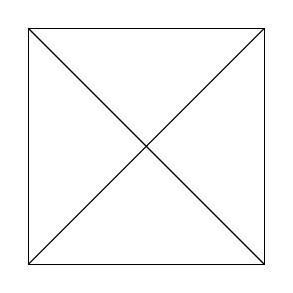
\begin{tikzpicture}
        \draw (0,0) rectangle (3,3);
        \draw (0,0)--(3,3);
        \draw (0,3)--(3,0);
    \end{tikzpicture}
    \end{minipage}
    \begin{minipage}[t]{0.45\textwidth}
    \centering
    \caption{错误的单形剖分}
    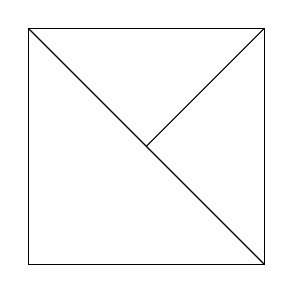
\begin{tikzpicture}
        \draw (0,0) rectangle (3,3);
        \draw (0,3)--(3,0);
        \draw (1.5,1.5)--(3,3);
    \end{tikzpicture}
    \end{minipage}
\end{figure}
有了空间划分$\mathscr{T}_{h}$后,定义在该划分空间上的分片多项式即可构成子空间$V_{h}\le V$。

